\section{Results}

    All results were generated by simulating a 200 satellite enviornment; 100 sensing satellites and 100 fusion nodes.
    The sensing satellites follow a 45 degree inclination, 1000 km altitude walker-delta constellation composed of 5 planes each with 20 satellites.
    Each sensing satellite has a bearings only sensor on it with a diagonal FOV of 115 degrees. Bearings measurements are taken as truth data of the target with added white noise of +- 0.115 degrees in either bearings angle direction (in-track angle and cross-track angle).
    The fusion satellites follow a 90 degree inclination, 1000 km altititude walker-delta constellation composed of 5 planes each with 20 satellites.
    Each fusion node has a maximum computational capacity of 2 tracks; meaning it can only handle 2 extended kalman filters at a time. 
    The communication network is a nearest neighbor network, with a maximum communication range of 1000 km and a maximum number of neighbors of 4.
    The scenario simulated has 5 countries spawning targets with random spherical dynamics: the United States, China, Ukraine, South Africa, and Argentina.

    The custody assignment MILP was reran every 1 minute in the simulation based on all avaliable target tracks throughout the fusion network.
    The planning horizon used for each MILP solution was also 1 minute.
    In scenarios where multiple fusion nodes have differenting target tracks, covariance intersection was used to reconcile the tracks, allowing planning under consistent knowledge.

\subsection{Undercapacity Case}

    % here show the results for how the milp performs in the undercapacity case. 

    % also show the scalability of the solver. 
    % a plot for time to solve solution and also a plot showing how the federated system performs.

    To test the performance of the MILP algorithm for a nominal, undercapacity case, each country was given 20 targets. 
    Every 1 minute in the simulation, a new custody plan was generated using the MILP algorithm. 
    The initial custody plan that was generated is shown in Figure~\ref{fig:initial_custody_nominal}.

    The targets are colored according to their country of origin, as shown in the legend.
    All sensing satellites are shown in a very dim blue, all fusion satellites without custody are shown in a very dim green. 
    The fusion satellites that were assigned custody of targets are colored the same as the targets they are assigned to.
    The black lines indicate communications of measurements on targets from the sensing layer to fusion nodes with custody.

    These results look to be succcessful, as all targets are being tracked by at least one fusion node. 
    Additionally, the fusion nodes that were assigned custody are close to the targets they were assigned, as optimized in the cost function. 
    This is able to reduce the amount of communication hops required for a measurement to reach the fusion node.
    
    We can also compare our solution from the MILP in a federated fusion architecture to that of a typical decentralized data fusion (DDF) architecture.
    Where in this typical DDF architecture, no custodies are assigned, instead, all fusion nodes run EKFs on every measurement they recieve. The sensing nodes send measurements they takes to the nearest fusion node in communication range.
    Thus, there is issues of track consistency in the network as you may have multiple fusion nodes tracking the same target using different measurements.
    This means that at each time step, the fusion nodes reconsile their independent tracks together using pairwise covariance intersection. 
    This pairwise covariance intersection was simulated alongside the federated MILP solution to see how the two architectures perform in the exact same scenarios.
    The results comparing the average fusion time of the per fusion node per time step are shown in Figure~\ref{fig:federated_vs_ddf}.

    \begin{figure}[h]
        \centering
        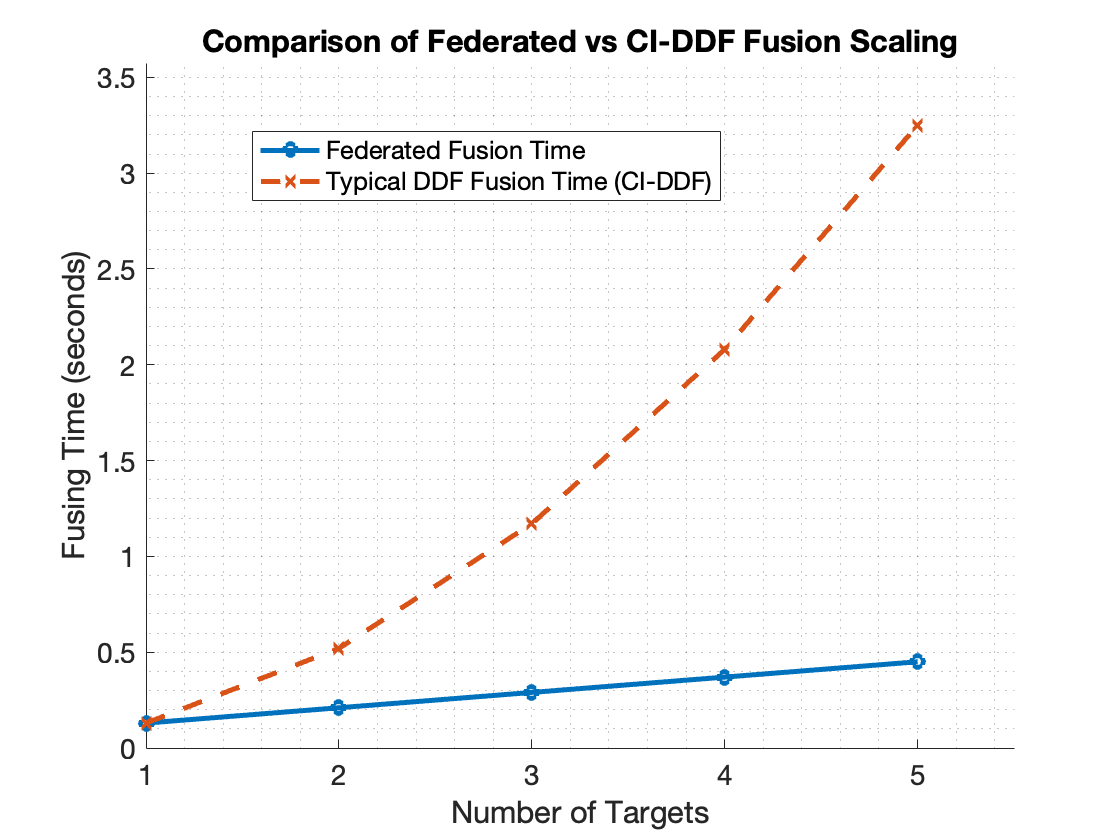
\includegraphics[width=0.5\textwidth]{figs/ci_vs_federated.png}
        \caption{Average fusion time per fusion node per time step for the federated MILP solution vs the CI DDF solution.}
        \label{fig:federated_vs_ddf}
    \end{figure}

    The results show a massive improvement to scalability when using the federated architecture with the MILP algorithm to assign custody. 
    The behavior of the DDF solution is about $O(N^2)$ with $N$ number of targets. This makes sense as each fusion node has to combine its tracks with neighboring fusion nodes each time step, leading to more communication and computation.
    The federated solution on the other hand is about $O(N)$ with $N$ number of targets. The custody-bounty system allows an average of 1 data fusion algorithm, such as an EKF, to be run per target, and little pairwsie fusion is required.

\subsection{Overcapacity Case}

    % show the plot of priority assignments vs exchange rate.
    % maybe show a plot showing how the system looks with a higher exchange rate?

    To test the performance of the MILP algorithm for an overcapacity case, each country was given 100 targets. 
    Additionally each country was assigned a priority, with the United States having a priority of 1, China having a priority of 2, Ukraine having a priority of 3, South Africa having a priority of 4, and Argentina having a priority of 5.

    For this overcapacity case, which targets the system chooses not to track is influenced heavily on the exchange rate, as formulated in Equation~\eqref{eq:exchange_rate}.
    Plots showing the custody assignments of the network for an exchange rate of 1 vs an exchange rate of 1.6 are shown in Figures~\ref{fig:exchange_rate_1} and \ref{fig:exchange_rate_1.6}.
    The relationship between the exchange rate and the number of targets tracked in each of the countries is shown in Figure~\ref{fig:assignment_vs_exchange_rate}.

    \begin{figure}[h]
        \centering
        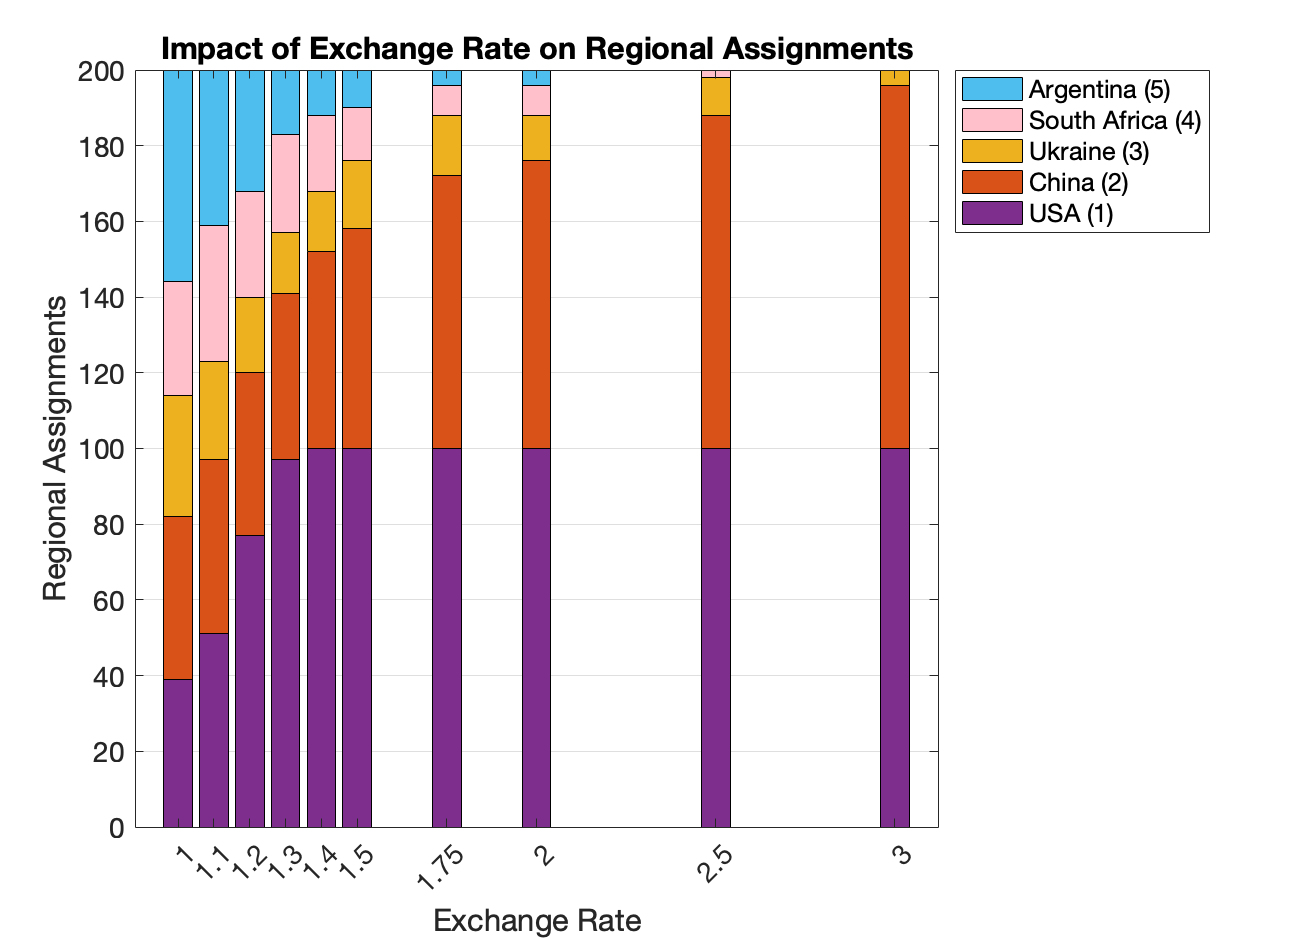
\includegraphics[width=0.5\textwidth]{figs/assignment_vs_exchange_rate.png}
        \caption{Relationship between number of targets tracked per country vs the exchange rate. Countries were given the priorities listed in the legend.}
        \label{fig:assignment_vs_exchange_rate}
    \end{figure}

    The results show that as the exchange rate increases in the system, the strength of the priorities in assigning targets increases. 
    This is a successful result as it shows the system is able to be adjusted to the needs of the user. 
    Depending on the exchange rate set by a user, the system can be adjusted to ensure the degredation in tracking targets matches the user's needs.

    However, it is important to note that by increasing the exchange rate and giving more weight to priorities, the system produces a worst result for minimizing communications. 
    The original MILP formulation wihtout priorities is design specifically to minimize communicaitons by using the proxy cost function given in Equation~\eqref{eq:cost}.
    By scaling this cost function with the priority factor, the solution is no longer optimal with resepct to that proxy function. 
    The relationship for the average communication distance travelled by a measurement through the network from sensing node to custody node is shown in Figure~\ref{fig:comm_distance_vs_exchange_rate}.

    \begin{figure}[h]
        \centering
        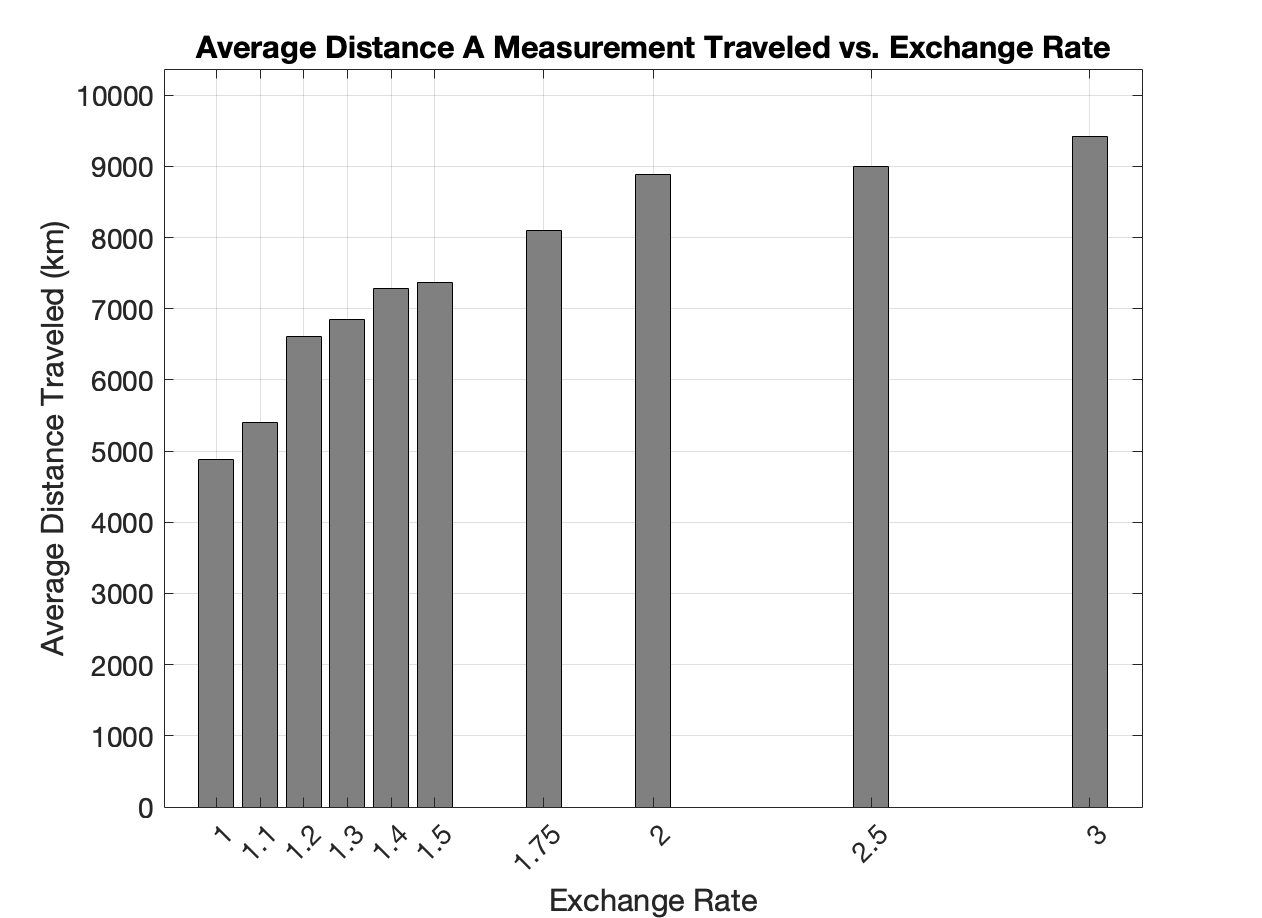
\includegraphics[width=0.5\textwidth]{figs/distance_vs_exchange.png}
        \caption{Average communication distance traveled by a measurement through the network from sensing node to custody node for a variety of exchange rates.}
        \label{fig:comm_distance_vs_exchange_rate}
    \end{figure}

    The results show for this overcapacity case, as the exchange rate increases, the average communication distance traveled by a measurement increases. 
    This result can be better visualized by looking at the custody plan for the exchange rates of 1 and 1.6, shown in Figures~\ref{fig:exchange_rate_1} and~\ref{fig:exchange_rate_1.6}.
    In these plots, you can see that at a higher exchange rate, the nodes assigned custody of the USA and China begin taking over the regions previously assigned to Argentina and South Africa. 
    While this happens due to the priority scaling, this decreases communication efficiency, thus, increasing latency and bandwidth usage. However, a higher number of higher priority targets are being tracked; 
    this is the resulting trade off that occurs when increasing the exchange rate. 

    A video showing the results of scaling the exchange rate online in the simulation environment is available at the top of the paper.